% This must be in the first 5 lines to tell arXiv to use pdfLaTeX, which is strongly recommended.
\pdfoutput=1
% In particular, the hyperref package requires pdfLaTeX in order to break URLs across lines.

\documentclass[11pt]{article}

% Remove the "review" option to generate the final version.
\usepackage[]{ACL2023}

% Standard package includes
\usepackage{times}
\usepackage{latexsym}

% For proper rendering and hyphenation of words containing Latin characters (including in bib files)
\usepackage[T1]{fontenc}
% For Vietnamese characters
% \usepackage[T5]{fontenc}
% See https://www.latex-project.org/help/documentation/encguide.pdf for other character sets

% This assumes your files are encoded as UTF8
\usepackage[utf8]{inputenc}

% This is not strictly necessary, and may be commented out.
% However, it will improve the layout of the manuscript,
% and will typically save some space.
\usepackage{microtype}

% This is also not strictly necessary, and may be commented out.
% However, it will improve the aesthetics of text in
% the typewriter font.
\usepackage{inconsolata}


% If the title and author information does not fit in the area allocated, uncomment the following
%
%\setlength\titlebox{<dim>}
%
% and set <dim> to something 5cm or larger.

\title{Extractive summarisation of biomedical research articles using TextRank, WordRank, and a hybrid approach}

% Author information can be set in various styles:
% For several authors from the same institution:
% \author{Author 1 \and ... \and Author n \\
%         Address line \\ ... \\ Address line}
% if the names do not fit well on one line use
%         Author 1 \\ {\bf Author 2} \\ ... \\ {\bf Author n} \\
% For authors from different institutions:
% \author{Author 1 \\ Address line \\  ... \\ Address line
%         \And  ... \And
%         Author n \\ Address line \\ ... \\ Address line}
% To start a seperate ``row'' of authors use \AND, as in
% \author{Author 1 \\ Address line \\  ... \\ Address line
%         \AND
%         Author 2 \\ Address line \\ ... \\ Address line \And
%         Author 3 \\ Address line \\ ... \\ Address line}

\author{Kristina Levina \\
  Course code: 732A81 \\
  \texttt{LiU-ID: krile102} \\}

\begin{document}
\maketitle
\begin{abstract}
This project aims at developing a tool to generate a summary automatically based on the main text of a biomedical research manuscript. To this end, extractive summarisation is employed. The motivation behind choosing extractive summarisation is, in essense, the neccessety to preserve the key sentences from the main text. Extractive summarisation will retrieve sentences based on their importance without rephrasing them, thereby excluding misinterpretations. This is crucial for scientific texts. In this project, SumPubMed dataset was used. According to the literature, SumPubMed dataset was created specifically for testing summarisation tools of biomedical research articles. Two algorithms were chosen to implement this task: TextRank as a baseline and a pretrained transformer from Hugging Face. Their performance was assessed using X and Y metrics. The obtained results show that Y better suits for the considered task. 

\end{abstract}

\section{Introduction}

With increasing volume of published articles in medical research, it becomes increasingly difficult for doctors, medical staff, and public health officials to stay updated. Sometimes, a

\section{Theory}
\subsection{PageRank}
\subsection{ROUGE}
\subsection{BLEU}

\section{Data}

\section{Method}
\subsection{TextRank}
\subsection{WordRank}
\subsection{Hybrid}

\section{Results}

\citet{reza2020}

\begin{figure}
 \centering
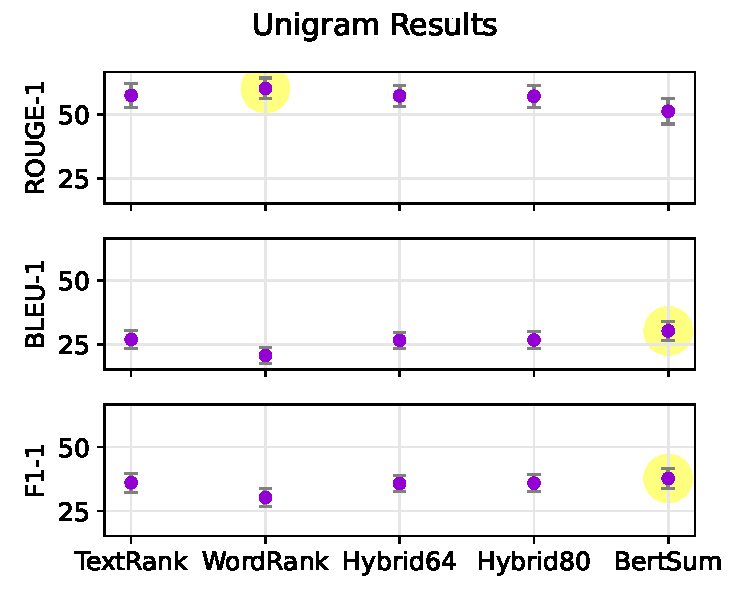
\includegraphics[scale=0.5]{unigrams.pdf}
\caption{An example graph}
\label{fig:x cubed graph}
\end{figure}


\section{Discussion}

\section{Conclusion}


% \begin{table}
% \centering
% \begin{tabular}{lc}
% \hline
% \textbf{Command} & \textbf{Output}\\
% \hline
% \verb|{\"a}| & {\"a} \\
% \verb|{\^e}| & {\^e} \\
% \verb|{\`i}| & {\`i} \\ 
% \verb|{\.I}| & {\.I} \\ 
% \verb|{\o}| & {\o} \\
% \verb|{\'u}| & {\'u}  \\ 
% \verb|{\aa}| & {\aa}  \\\hline
% \end{tabular}
% \begin{tabular}{lc}
% \hline
% \textbf{Command} & \textbf{Output}\\
% \hline
% \verb|{\c c}| & {\c c} \\ 
% \verb|{\u g}| & {\u g} \\ 
% \verb|{\l}| & {\l} \\ 
% \verb|{\~n}| & {\~n} \\ 
% \verb|{\H o}| & {\H o} \\ 
% \verb|{\v r}| & {\v r} \\ 
% \verb|{\ss}| & {\ss} \\
% \hline
% \end{tabular}
% \caption{Example commands for accented characters, to be used in, \emph{e.g.}, Bib\TeX{} entries.}
% \label{tab:accents}
% \end{table}



\section{Preamble}
\begin{table*}
\centering
\begin{tabular}{lll}
\hline
\textbf{Output} & \textbf{natbib command} & \textbf{Old ACL-style command}\\
\hline
\citep{ct1965} & \verb|\citep| & \verb|\cite| \\
\citealp{ct1965} & \verb|\citealp| & no equivalent \\
\citet{ct1965} & \verb|\citet| & \verb|\newcite| \\
\citeyearpar{ct1965} & \verb|\citeyearpar| & \verb|\shortcite| \\
\citeposs{ct1965} & \verb|\citeposs| & no equivalent \\
\citep[FFT;][]{ct1965} &  \verb|\citep[FFT;][]| & no equivalent\\
\hline
\end{tabular}
\caption{\label{citation-guide}
Citation commands supported by the style file.
The style is based on the natbib package and supports all natbib citation commands.
It also supports commands defined in previous ACL style files for compatibility.
}
\end{table*}
% The first line of the file must be
% \begin{quote}
% \begin{verbatim}
% \documentclass[11pt]{article}
% \end{verbatim}
% \end{quote}






Table~\ref{citation-guide} shows the syntax supported by the style files.
We encourage you to use the natbib styles.
You can use the command \verb|\citet| (cite in text) to get ``author (year)'' citations, like this citation to a paper by \citet{Gusfield:97}.
You can use the command \verb|\citep| (cite in parentheses) to get ``(author, year)'' citations \citep{Gusfield:97}.
You can use the command \verb|\citealp| (alternative cite without parentheses) to get ``author, year'' citations, which is useful for using citations within parentheses (e.g. \citealp{Gusfield:97}).




% Entries for the entire Anthology, followed by custom entries
\bibliography{custom}
\bibliographystyle{acl_natbib}


\end{document}
